% IEEEAerospace2012.cls requires the following packages: times, rawfonts, oldfont, geometry
\documentclass[twocolumn,letterpaper]{IEEEAerospaceCLS}  % only supports two-column, letterpaper format

% The next line gives some packages you may find useful for your paper--these are not required though.
%\usepackage[]{graphicx,float,latexsym,amssymb,amsfonts,amsmath,amstext,times,psfig}
% NOTE: The .cls file is now compatible with amsmath!!!

\usepackage[]{graphicx}    % We use this package in this document
% \usepackage{cite}
\usepackage[backend=biber, style=ieee]{biblatex} %Imports biblatex package
\addbibresource{DOJO_CKC_IEEE_AERO.bib}
\usepackage{amsmath,amssymb,amsfonts}
\usepackage{algorithmic}
\usepackage{textcomp}
\usepackage{xcolor}
% \usepackage[disable]{todonotes}
\usepackage{comment}
\usepackage{optidef}
\usepackage{pgfplots}
\usepackage{svg}
\usepackage{url}
% \usepackage{tikz}
\usepackage[justification=justified,singlelinecheck=false]{caption}

\pgfplotsset{compat=1.18} 
% \excludecomment{figure}
% \excludecomment{figure*}
% \excludecomment{todo}
% \let\endfigure\relax
% \let\endfigure*\relax
\newcommand{\ignore}[1]{}  % {} empty inside = %% comment
\newcommand{\todo}[1]{\textcolor{red}{TODO: #1}}


\begin{document}
\title{Data-Driven Physics-Based Digital Twin \\
for Linkage Analysis}

\author{%
Mitchell Fogelson\\ 
Carnegie Mellon University\\
5000 Forbes Ave\\
Pittsburgh PA, 15213\\
mfogelson@cmu.edu
\and 
Zachary Manchester\\
Carnegie Mellon University\\
5000 Forbes Ave\\
Pittsburgh PA, 15213\\
zacm@cmu.edu
%%%% IMPORTANT: Use the correct copyright information--IEEE, Crown, or U.S. government. %%%%%
\thanks{\footnotesize 979-8-3503-5597-0/25/$\$31.00$ \copyright2025 IEEE}              % This creates the copyright info that is the correct 2025 data.
%\thanks{{U.S. Government work not protected by U.S. copyright}}         % Use this copyright notice only if you are employed by the U.S. Government.
%\thanks{{979-8-3503-5597-0/25/$\$31.00$ \copyright2025 Crown}}          % Use this copyright notice only if you are employed by a crown government (e.g., Canada, UK, Australia).
%\thanks{{979-8-3503-5597-0/25/$\$31.00$ \copyright2025 European Union}}    % Use this copyright notice is you are employed by the European Union.
}


\maketitle
% \begin{abstract}
Linkage mechanisms are fundamental in the design of deployable space structures, enabling efficient packing and significant expansion. However, they have a high risk of jamming and are a source of single-point failures. 
% Extensive testing is essential for ensuring mission success, but it is often time-consuming and resource intensive. 
Simulation tools provide a viable method to increase confidence of mission success, offering insights into system behavior without relying on physical prototypes. However, rigid-body dynamic simulations struggle to capture the effects of joint clearance and friction. 
% Digital twins combine hardware data with physics engines, expediting the testing process and improving the accuracy of reduced-order models.
This paper implements a data-driven, physics-based digital-twin framework for linkage analysis. Our approach uses a differentiable physics engine and real data from hardware experiments to estimate joint clearance and friction for a target mechanism.
%The differentiable physics engine uses a “maximal coordinates” representation where each link’s full pose in SE(3) is explicitly defined, and joint constraints are applied directly. 
% Using singular value decomposition (SVD), we eliminate redundant constraints, allowing the simulation to step through only the unconstrained degrees of freedom in the system.
%This approach enables accurate simulation of complex linkages with joint clearances and friction.
We validate our approach using both synthetic data and a hardware experiment on a multi-cell scissor mechanism. Our model correctly captures linkage jamming due to joint clearance and friction and closely matches trajectories captured during hardware experiments. 

% Initial hardware results are presented on a scissor mechanism with 23 units, where the digital twin shows qualitatively similar behaviors and an average linked error of less than 2cm.
% \end{abstract} 
\tableofcontents
%%%%%%%%%%%%%%%%%%%%%%%%%%%%%%%%%%%%%%
\section{Introduction} \label{intro}
%%%%%%%%%%%%%%%%%%%%%%%%%%%%%%%%%%%%%%
% \todo{
% \begin{enumerate}
%     \item Fix Mitch's headshot photo
%     \item revolute joint constraint definition
%     \item emphasize that we use data to capture the hardest-to-model parts of the system: joint friction and tolerancing/slop/clearance
% \end{enumerate}
% }
\begin{figure}
    %\centering
    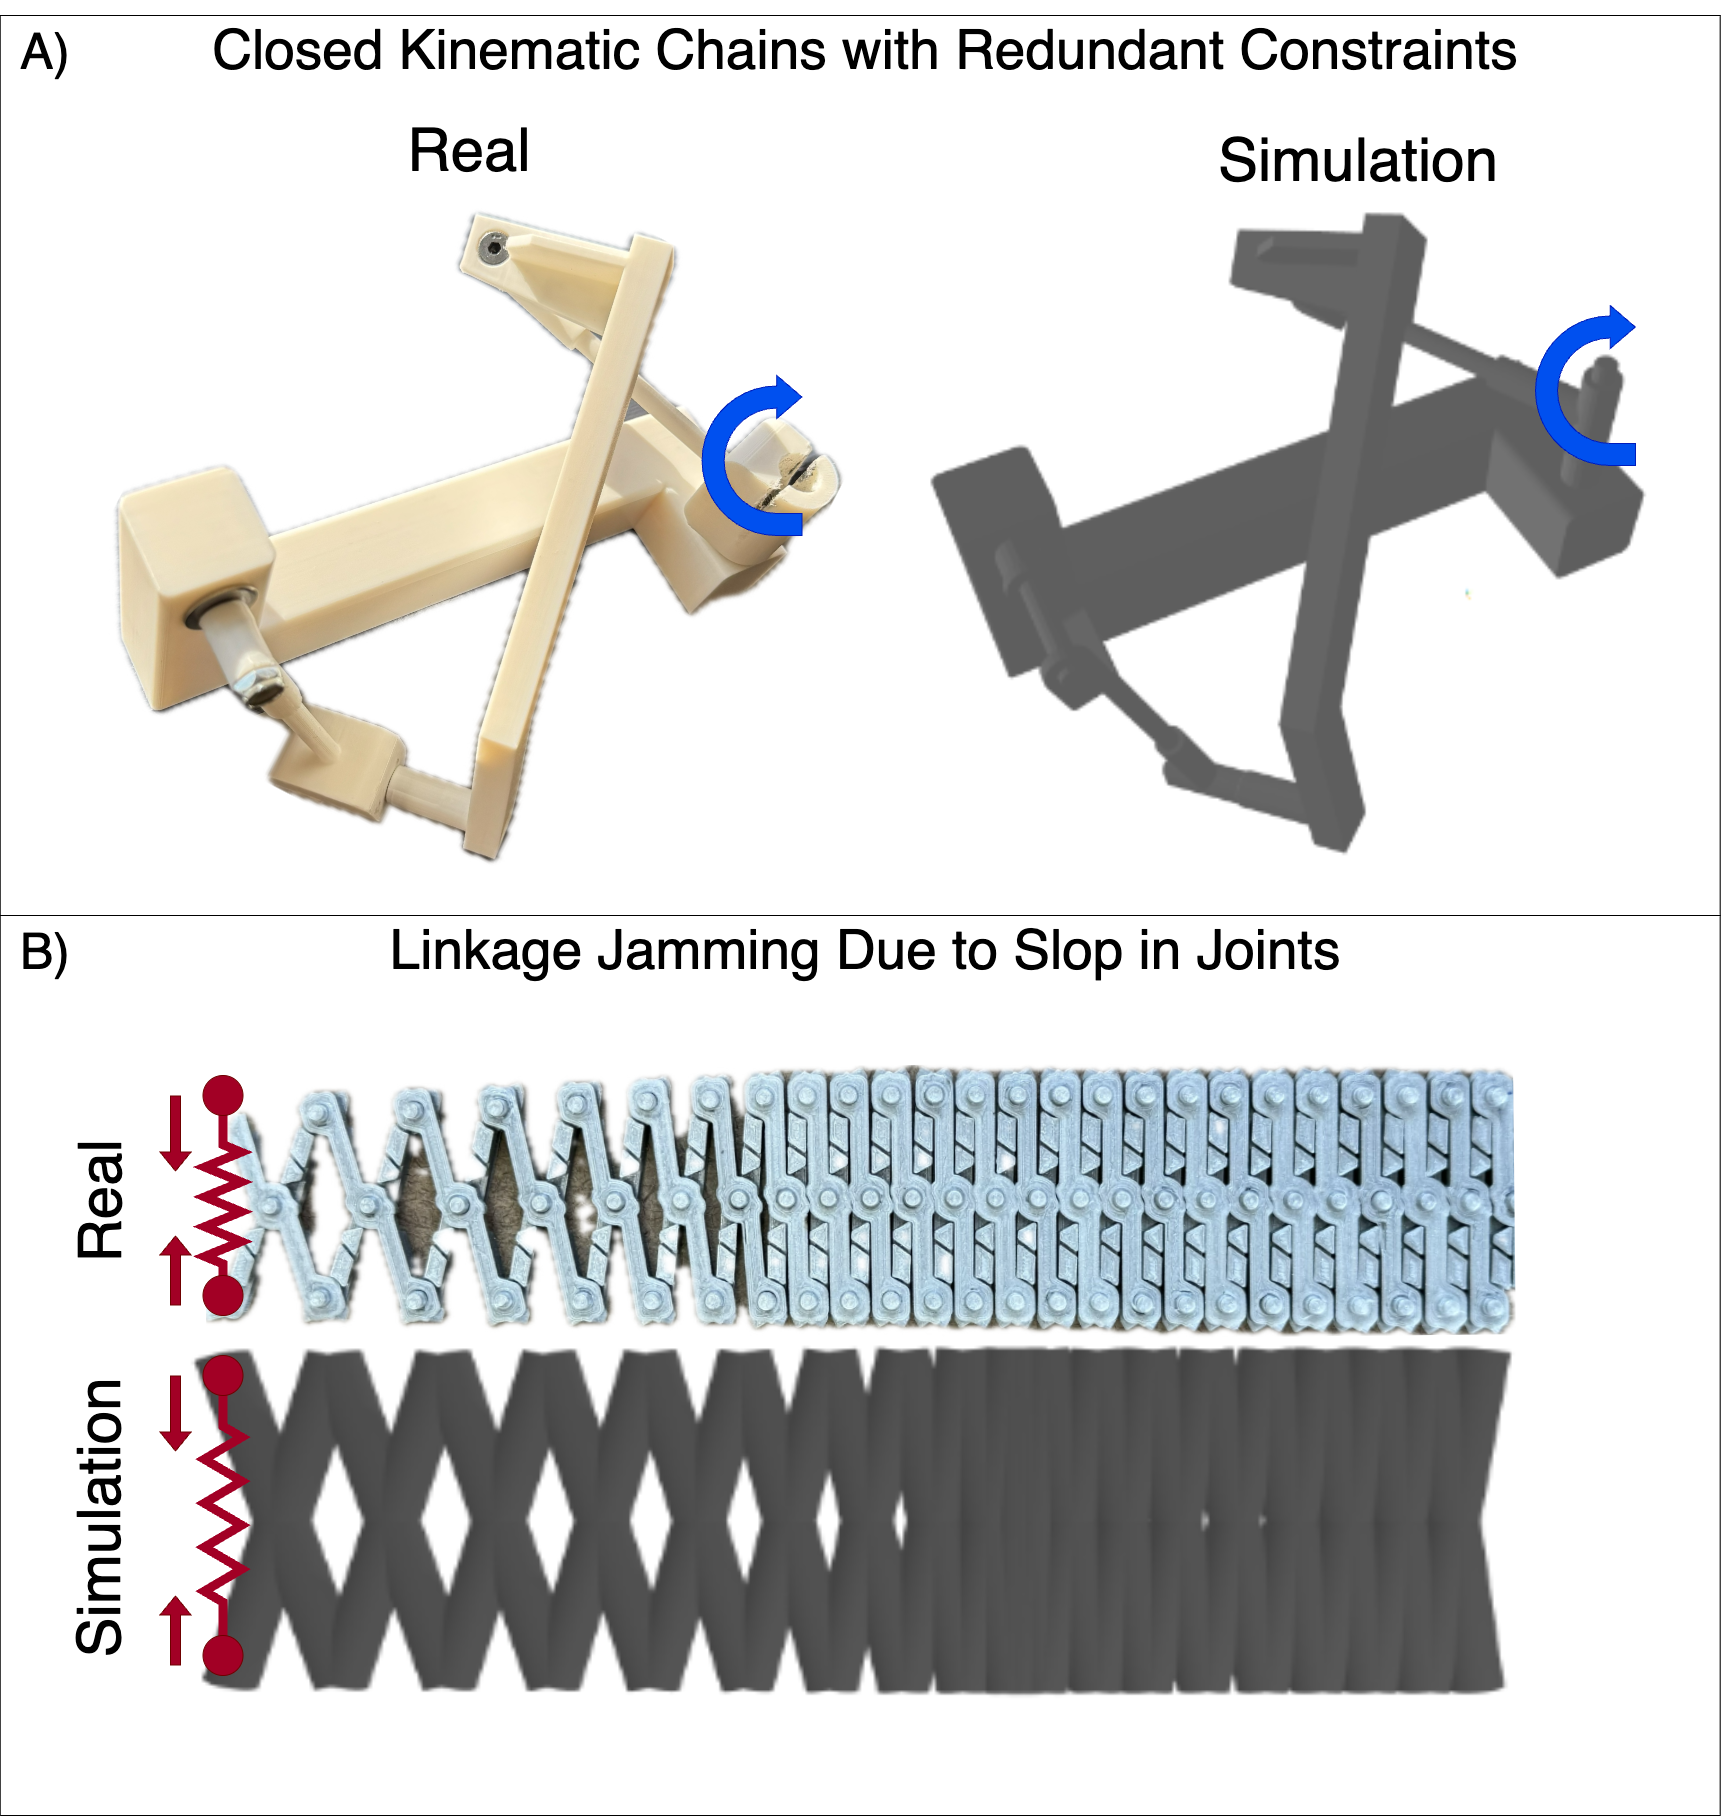
\includegraphics[width=\linewidth]{DOJO-CCK/Figures/scissor_slop.drawio.png}
    \caption{Two examples of complex mechanisms—(A) a Bennett linkage and (B) a jamming scissor mechanism—demonstrating both real and simulated models. These mechanisms' joint clearance and friction can be characterized through a digital twin pipeline, which improves model predictiveness. Our system leverages sensor data from physical prototypes alongside a physics engine, allowing it to learn key parameters such as joint slop and dynamic interaction, enabling accurate simulations and predictive modeling of mechanical behavior.}
    \label{fig:Hero-Figure}
\end{figure}
Linkage mechanisms play a crucial role in the design of deployable space structures, as demonstrated by the intricate mechanisms used in the James Webb Telescope (JWST). The JWST features highly complex deployment mechanisms designed to pack into the Ariane 5 rocket and deploy when released into space. However, these mechanisms introduce significant risks, with some estimates identifying 344 potential single-point failures \cite{menzel_lessons_2024}. Ensuring the success of such a mission necessitates extensive testing, which is time consuming and resource intensive. With systems like the JWST, failure of linkage deployment is one of the aspects tested intensely on Earth before launch. While JWST was successful, Rivera et al. reviewed failures in spacecraft deployable systems in many other instances and cited jamming due to linkage friction or unexpected loads as key examples \cite{rivera_study_2021}. 

Simulation tools offer a valuable resource that allows engineers to analyze system behavior without physical prototypes. Recent advancements in robotics simulation, exemplified by software tools like MuJoCo \cite{todorov_mujoco_2012} and Isaac Sim \cite{mittal_orbit_2023}, have significantly enhanced engineers’ ability to test designs and control algorithms before risking hardware. However, these simulations often fail to fully capture real-world behavior, commonly referred to as the ``sim-to-real gap.''

One solution to the sim-to-real gap is digital twins, which integrate data from the physical world, enabling feedback between the physical system and its virtual counterpart \cite{tao_digital_2019}. Using real-world data with machine-learning algorithms and/or advanced modeling techniques, digital twins provide a more accurate representation of the system in operation \cite{phanden_review_2021}. This synchronization allows engineers to refine simulations, account for unexpected variations, and optimize control or design \cite{ritto_digital_2021, kapteyn_data-driven_2022}. Consequently, digital twins have the potential to play a crucial role in enhancing the fidelity and reliability of linkage-based systems across various development stages.

A key challenge for rigid-body simulators is handling linkages with redundant constraints, joint clearance, and joint friction, which leads to the need for bespoke solutions for complex linkages. Redundant constraints can cause numerical instability, making accurate simulation difficult. Prior work from Wojtyra et al.,  provided analytic conditions for determining uniquely solvable reaction forces in systems with redundant nonholonomic constraints \cite{wojtyra_joint_2009}. Wojtyra et al., later presented a mathematical framework for identifying and calculating joint reactions in mechanisms with dependent constraints due to redundancy or singular configurations \cite{wojtyra_solvability_2013}. To reduce the ill-conditioning, Pekal et al., compared several numerical approaches such as SVD, QR, and nullspace methods \cite{pekal_constraint-matrix-based_2023}. 

In addition, joint friction and joint clearances --- also called ``slop'' or ``tolerance'' --- that arise from manufacturing errors or mechanism wear limit the accuracy of existing simulators. Prior work has explored improving the dynamic modeling of specific linkage configurations with joint clearance \cite{funabashi_dynamic_1978, soong_theoretical_1990} but fail to extend to general linkages.  More recent work has focused on contact force modeling and characterizing the influence on linkage operation \cite{akhadkar_influence_2014, tan_continuous_2017}. In a different approach, some prior work explicitly includes joint clearances into the design process, where they then evaluate linkage trajectory purely kinematically  \cite{mutawe_designing_2012, qi_synthesis_2023}.

% Funabashi et al. systematically analyzed the dynamic behavior of multilink mechanisms with joint clearances, incorporating elastic deformations and friction \cite{noauthor_dynamic_nodate}. Soong et al. developed an analytical model to predict the dynamic behavior of a slider-crank mechanism with radial clearance in its joints \cite{soong_theoretical_1990}. Akhadkar et al. analyzed the impact of joint clearances on the performance of multibody systems by modeling the contact forces in pin and hole assemblies \cite{Akhadkar_influence_2014}. Tan et al. developed a continuous analysis method to investigate dynamic responses in planar mechanisms with clearance, focusing on how joint contact and friction influence the system's motion \cite{tan_continuous_2017}. Mutawe et al. addressed path generation for four-bar linkages under joint clearance constraints and developed a design synthesis method that accounted for joint tolerances, ensuring that mechanisms could achieve specified paths within defined tolerance limits\cite{mutawe_designing_2012}. Qi et al. proposed a method to introduce joint clearances in overconstrained linkages to prevent jamming due to component deformation \cite{qi_synthesis_2023}.  Dupont et al. explored the relationship between Coulomb friction and jamming in rigid-body dynamics \cite{dupont_jamming_1994}. 

While previous work has focused on theoretical outcomes or the characterization of specific linkage configurations~\cite{funabashi_dynamic_1978, soong_theoretical_1990, dupont_jamming_1994, akhadkar_influence_2014, tan_continuous_2017}, this paper introduces a generalizable framework for creating digital twins for linkage analysis. Our approach extends traditional rigid body dynamics simulations by incorporating data-driven parameter estimation from the target mechanism. The proposed framework integrates computer-aided design (CAD), a differentiable simulator, and real-world data to build a data-driven, physics-based digital twin for linkage mechanisms. From the CAD software, the linkage is exported, along with its geometry and physical properties, into a differentiable physics engine that operates using maximal coordinates. Redundant constraints are removed systematically through singular-value decomposition (SVD). Real-world position data is then used to fit joint clearance and damping values for dynamic analysis. These fit parameters are applied in simulations to evaluate system behavior under unseen loads, including detecting jamming. We demonstrate this approach with both simulated and real examples of multi-link scissor mechanisms, as shown in Figure \ref{fig:Hero-Figure}.
% While prior work focused on theoretical results or the characterization of specific linkage configurations, this work presents a generalizable framework for creating digital twins for linkage analysis. Our work extends on a nominal rigid body dynamics simulation through data-driven parameter estimation from target mechanism data. The framework presented in this paper combines computer-aided design (CAD), a differentiable simulator, and real-world data to develop a data-driven physics-based digital twin for the linkage mechanism. A CAD-designed linkage is exported with geometry and physical parameters to a modified differentiable physics engine using maximal coordinates. Redundant constraints are systematically removed via singular value decomposition (SVD). Real-world position data enables optimization of joint clearance and damping for dynamic analysis. These parameters are then applied to simulate the system under unseen loads, evaluating potential jamming scenarios that can be detected through the SVD. We demonstrate our approach using simulated and real examples of multi-link scissor mechanisms seen in Figure \ref{fig:Hero-Figure}.

% Our methodology enables dynamic simulation of linkages with many redundant constraints, providing a robust framework for analyzing and designing complex mechanisms like those found in the JWST. We demonstrate our approach on several interesting linkage examples including several scissor mechanism variants, the Jansen linkage, and a hierarchical linkage mechanism combining a Kresling and scissor system together. 

% Furthermore, our approach allows us to investigate the impact of manufacturing tolerances on linkage performance. Specifically, we can simulate how slight variations in manufacturing can lead to linkage jamming, a critical concern for the reliability of space mechanisms. By understanding these effects, we can propose pathways for designing more robust linkage configurations that are less susceptible to tolerancing-induced failures.

The specific contributions of this work are: 
\begin{enumerate}
    \item A data-driven physics-based digital twin framework for linkage mechanisms that capture joint clearance and joint friction effects 
    \item Analysis of linkage jamming and joint reaction forces 
    % \item An approach to improve the numerical conditioning of the simulation that occurs from redundant linkage constraints through SVD system reduction
    \item Hardware validation of linkage digital twins 
\end{enumerate}

This paper proceeds as follows: Section \ref{background} provides information on the ``maximal coordinate'' simulation representation, joint constraints, and SVD factorization. Section \ref{method} describes the digital twin pipeline that combines the simulator and real-world data. Section \ref{experiments} describes the simulation-based and hardware experiments to verify our approach. Then, Section \ref{results} presents the results and findings of this digital twin for linkages. Finally, Section \ref{conclusion} summarizes our findings, presents the limitations of the work, and makes suggestions for the system's future development. % % \section{Related Works} \label{related}
% A variety of works have looked into various methods of rigid body dynamics for simulating closed-loop linkages, how to address the numerical issues of redundant constraints that arise in these problems, as well as how joint clearance can effect these linkage systems. 

% \subsection{Redundant Constraints}

% Muller's work explored the concept of generic degrees of freedom (DOF) in mechanisms, showing how imperfections in link geometry impact mobility \cite{muller_generic_2009}. The author demonstrated that most mechanisms are not overconstrained and have predictable DOFs, making it easier to classify mechanisms as overconstrained, underconstrained, or kinematotropic. Wojtyra et al.,  provided analytic conditions for determining uniquely solvable reaction forces in systems with redundant nonholonomic constraints \cite{wojtyra_joint_2009}. They developed numerical methods to detect constraints that allow for unique solutions, contributing to a more accurate modeling of constrained multibody systems. Wojtyra et al., later presented a mathematical framework for identifying and calculating joint reactions in mechanisms with dependent constraints due to redundancy or singular configurations. It showed how specific joint reactions could be uniquely determined despite the overall indeterminacy of the system \cite{wojtyra_solvability_2013}. Pekal et al., compared several numerical approaches—SVD, QR, and nullspace methods—and demonstrated how to check the uniqueness of selected forces within multibody systems efficiently \cite{pekal_constraint-matrix-based_2023}.

% \subsection{Joint Clearance Analysis}

% Funabashi et al. systematically analyzed the dynamic behavior of multilink mechanisms with joint clearances, incorporating elastic deformations and friction. The paper revealed how clearances and crank speeds affect the relative motion, input torque, and output displacement of mechanisms \cite{noauthor_dynamic_nodate}. Soong et al. developed an analytical model to predict the dynamic behavior of a slider-crank mechanism with radial clearance in its joints \cite{soong_theoretical_1990}. Akhadkar et al. analyzed the impact of joint clearances on the performance of multibody systems by modeling the contact forces in pin and hole assemblies. It demonstrated how even small clearances degrade the performance of mechanisms, particularly at lower input speeds \cite{Akhadkar_influence_2014}. Tan et al. developed a continuous analysis method to investigate dynamic responses in planar mechanisms with clearance joints, focusing on how joint contact and friction influence the system's motion \cite{tan_continuous_2017}. 

% Mutawe et al. addressed path generation for four-bar linkages under joint clearance constraints, incorporating ANSI tolerance standards. The authors developed a design synthesis method that accounted for joint tolerances, ensuring that mechanisms could achieve specified paths within defined tolerance limits\cite{mutawe_designing_2012}. Qi et al. proposed a method to introduce joint clearances in overconstrained linkages to prevent jamming due to component deformation. Their model optimizes clearance placement to ensure smooth mechanism operation under deformation \cite{qi_synthesis_2023}.

% \subsection{Jamming and Failure}
% Dupont et al. explored the relationship between Coulomb friction and jamming in rigid-body dynamics. They provided conditions for jamming and wedging in constrained systems, illustrating their findings with practical examples \cite{dupont_jamming_1994}. Rivera et al., reviewed failures in spacecraft deployable systems, particularly focusing on solar arrays and antennas. The analysis identified common causes of deployment failures and suggested best practices for future designs to mitigate the risks of jamming and other deployment issues \cite{rivera_study_nodate}.


%%%%%%%%%%%%%%%%%%%%%%%%%%%%%%%%%%%%%%
\section{Background} \label{background}
%%%%%%%%%%%%%%%%%%%%%%%%%%%%%%%%%%%%%%
% \begin{figure}
%     \centering
%     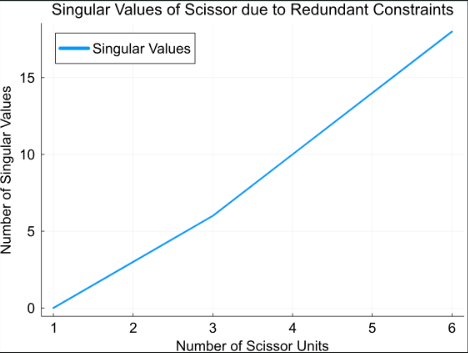
\includegraphics[width=\linewidth]{DOJO-CCK/Figures/singular_values_scissor.png}
%     \caption{The growth of singular values for scissor mechanism}
%     \label{fig:singular-vals}
% \end{figure}
% \includegraphics[width=\linewidth]{example-image-a}
This section briefly reviews multi-body dynamics with constraints and the singular-value decomposition (SVD).

\subsection{Dynamics} We leverage a differentiable physics engine, Dojo \cite{howell_dojo_2022}, which is based on “maximal coordinates,” in which each link is parameterized by its full SE(3) pose, and joints are represented with explicit constraints. The maximal-coordinate dynamics are described by:
\begin{equation}
\textbf{x} = \begin{bmatrix}
    \textbf{x}_1 \\
    \vdots \\
    \textbf{x}_n
\end{bmatrix}, \ \textbf{x}_i = \begin{bmatrix}
    \textbf{r}_i \\ \textbf{q}_i \\ \textbf{v}_i \\ \boldsymbol{\omega}_i
\end{bmatrix},    \dot{\textbf{x}} = \begin{bmatrix}
    \dot{\textbf{x}}_1 \\ 
    \vdots \\ 
    \dot{\textbf{x}}_n
\end{bmatrix}
% \label{eq:space_struct1}
\end{equation}
\begin{equation}
    \dot{\textbf{x}}_i = \begin{bmatrix}
    {\textbf{v}}_i \\ \frac{1}{2}\textbf{q}_i \otimes \boldsymbol{\omega}_i \\ M_i^{-1} \cdot (\textbf{f}_{\text{ext}, i} + \textbf{f}_{\text{int}, i}) \\ J_i^{-1} \cdot (\boldsymbol{\tau}_{\text{ext}, i} + \boldsymbol{\tau}_{\text{int}, i} - \boldsymbol{\omega}_i \times J_i \cdot \boldsymbol{\omega}_i)
\end{bmatrix}  
\end{equation}
\begin{equation}
    \begin{bmatrix}
    \textbf{f}_{int} \\
    \boldsymbol{\tau}_{int}
\end{bmatrix}  = \frac{\delta c(\textbf{x})}{\delta \textbf{x}}^T\boldsymbol{\lambda}
\end{equation}
% \begin{equation}
%      \textbf{f}_{\text{ext}, i} = \textbf{u}_{f,i} + M_i \cdot \textbf{g}, \quad \textbf{f}_{\text{int}, i} = -K_x \Delta \textbf{p}_{ij} - C_x \Delta \textbf{v}_{ij}
%      \label{eq:space_struct2}
% \end{equation}
% \begin{equation}
%     \boldsymbol{\tau}_{\text{ext}, i} = \textbf{u}_{\tau,i} + \textbf{p}_i \times \textbf{q}_i \otimes (\textbf{f}_{\text{ext}, i} + \textbf{f}_{\text{int}, i})
%     \label{eq:space_struct3}
% \end{equation}
% \begin{equation}
%     \boldsymbol{\tau}_{\text{int}, i} = -K_t \Delta \boldsymbol{\phi}_{ij} - C_t \Delta \boldsymbol{\omega}_{ij} 
% \end{equation}
where \(\textbf{r}_i \in {{\mathbb{R}}^3}\) represents the position vector for each body, \(\textbf{q}_i\in {{\mathbb{H}}}\) is the quaternion representing orientation of the body, \(\textbf{v}_i \in {{\mathbb{R}}^3}\) is the linear velocity, and \(\boldsymbol{\omega}_i \in {{\mathbb{R}}^3}\) is the angular velocity of each body. The mass matrix of a body is \(M_i\), and the inertia matrix is \(J_i\). Finally, the holonomic constraints, such as joints, are represented by $c(\textbf{x})$. The Lagrange multipliers $\boldsymbol{\lambda}$ represent the constraint forces and torques that satisfy these constraints. 

Representing a linkage mechanism using maximal coordinates offers several advantages: First, it avoids the challenges of defining generalized coordinates for closed kinematic chains, especially as linkage complexity grows. Second, using maximal coordinates makes representing joint clearances with inequality constraints straight forward. Finally, maximal coordinates provide direct correlations between joint-constraint values and the forces and torques acting on the body, offering clearer insight into the load distribution across linkage members. 

\subsection{Joint Constraints}
Incorporating joint constraints using Lagrange multipliers is a key technique in multibody dynamics, as it integrates constraints directly into the equations of motion. Lagrange multipliers introduce additional variables that represent the forces or torques necessary to enforce the joint conditions.
\begin{figure}
    \centering
    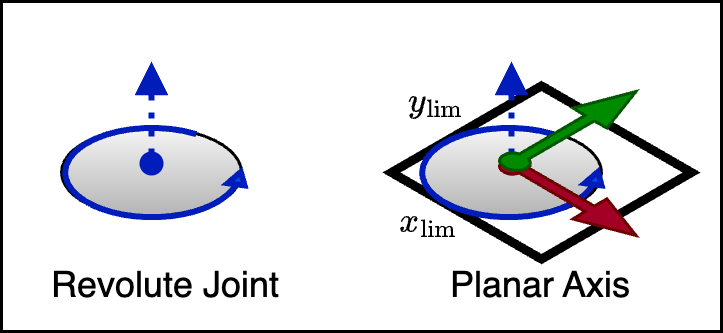
\includegraphics[width=0.8\linewidth]{Figures/joint_description.drawio.png}
    \caption{Diagrams of revolute and planar axis joint prototypes that are used to construct mechanism with clearance.}
    \label{fig:joint-proto}
\end{figure}
This work primarily deals with revolute joint-based mechanisms with joint clearance,  which is described using a planar-axis joint seen in Figure \ref{fig:joint-proto}. This joint allows the bodies to translate freely within a prescribed rectangular area with respect to each other. 

Although this approach is geometrically imprecise, the constraint typically positions the bodies near the corners of the rectangular constraint boundary, where the constraint forces are a linear combination of the adjacent sides. As a result, the force distribution closely resembles that of circular or elliptical constraints. The planar-axis joint was selected due to the current implementation in Dojo. Future work will explore more accurate joint constraints that better reflect the actual clearances in linkage mechanisms.

\subsection{Singular Value Decomposition}\label{sec:svd}
Singular Value Decomposition (SVD) is a powerful linear algebra technique widely used in model reduction to simplify complex systems while retaining essential dynamic features. SVD decomposes a matrix into three factors: 
\begin{equation}
    USV = \operatorname{SVD}(A)
\end{equation}
% \begin{equation}
%     A = USV^T
% \end{equation}
where $U$ is an orthogonal matrix of left singular vectors, $S$ is a diagonal matrix of singular values, and $V$ is an orthogonal matrix of right singular vectors. In the context of model reduction, SVD identifies the most significant modes of a system by ranking the singular values, which represent the importance or energy contribution of each mode. By truncating smaller singular values, we can create a reduced-order model that approximates the original system without the ill-conditioning from redundant, constrained degrees of freedom:
\begin{equation}
    \Tilde{A} = U[:, 1:r]S[1:r, 1:r]V[:,1:r]^T ,
\end{equation}
where $\Tilde{A}$ is the approximated rank-reduced matrix with rank $r$. Importantly for us, the SVD can factorize rectangular and rank-deficient matrices and is numerically robust.  

% This approach is particularly beneficial in large-scale linkage analysis, where computational efficiency is critical without sacrificing accuracy.

% Closed loop mechanisms suffer from numerical instability brought through redundant constraints. Our method systematically removes redundant constraints by using a singular value decomposition (SVD), resulting in a numerically robust method that takes steps only in the instantaneously unconstrained degrees of freedom of the system.

%%%%%%%%%%%%%%%%%%%%%%%%%%%%%%%%%%%%%%
\section{Method} \label{method}
%%%%%%%%%%%%%%%%%%%%%%%%%%%%%%%%%%%%%%
\begin{figure*}
    \centering
\includegraphics[width=\textwidth]{DOJO-CCK/Figures/block_diagram.drawio.pdf}
    \caption{A block diagram illustrating the data-driven, physics-based digital twin pipeline for linkage analysis. The process begins with a CAD model, exported to the physics engine for rigid body simulation. Simultaneously, real-world data is captured through various sensors (e.g., video, motion capture, and other sensing technologies) and synthesized using methods like optical flow or Kalman filters to estimate joint positions. The synthesized data undergoes kinematic analysis to estimate joint clearance, followed by dynamic analysis to estimate joint friction. These parameters are fed back into the physics engine for downstream analysis, including simulations of unseen loading conditions, jamming detection, and evaluating force/torque requirements.}
    \label{fig:block-diagram}
\end{figure*}

This section describes a method for creating a data-driven, physics-based digital twin for linkage analysis. A block diagram of the full process can be seen in Fig. \ref{fig:block-diagram}. The digital twin starts with designing the mechanism in CAD software, where it is then exported and parsed into Dojo \cite{howell_dojo_2022}, a maximal coordinate physics engine. The linkage is manufactured where imperfections introduce unknown parameters like joint clearance and joint friction. Data is collected on real deployments, and joint parameters are estimated through a kinematic and dynamic analysis facilitated by the physics engine to minimize motion errors between the real and simulation components. Finally, downstream analysis of unseen loading conditions can be evaluated in the digital twin, for example, if linkage jamming occurs. The following subsections go into greater depth on these subtasks.   

\subsection{System Modeling in CAD}

Leveraging design and modeling tools like CAD is crucial to creating a generalizable digital twin for linkages. Compared to the often labor-intensive process of designing complex systems purely through code, these tools provide a more efficient and accurate way to capture geometry, material properties, and relationships between bodies. In this work, the mechanism is modeled using Autodesk Fusion 360 \cite{autodesk_fusion_2014}, where individual components are assembled using fixed and revolute joints to capture the physical constraints of the system. Through the Fusion 360 Python API, each component's geometry, position, orientation, mass, inertia properties, and joint definitions are exported. While the current exporter supports only fixed and revolute joints, it can be extended to accommodate other joint types in future work.

\subsection{Maximal Coordinate Representation Parsing}

The exported data is converted into a maximal coordinate representation compatible with the Dojo mechanism description. Dojo is a differentiable rigid body simulation that uses a variational integrator and interior point method to provide high accuracy on inequality constraints while maintaining smooth gradients \cite{howell_dojo_2022}. However, using Dojo out of the box on closed-loop mechanisms like multi-cell scissors will lead to numerical ill-conditioning and failure. As mentioned in Section \ref{sec:svd}, the SVD factorization allows for general factorization of the system, systematically removing redundant constraints. The threshold for truncating singular values in SVD was set at \(10^{-7}\), determined through trial and error. Future research will explore automatic threshold selection based on eigenvalue patterns.

\subsection{Data Capturing and Synthesis}

Integrating real-world data into the physics engine is essential for developing more effective digital twins. This data can be gathered from various sensors and modalities. This work used a vision-based sensor system and position-based state estimation. The physical model was enhanced with high-contrast colored markers placed on the joints of the scissor mechanism. Linkage data was captured using an iPhone camera recording in slow motion at 240fps. OpenCV \cite{itseez_open_2015}, along with Meta's Co-Tracker\cite{karaev_cotracker_2023}—a deep learning-based optical flow method—was used to track the pixel locations corresponding to the rigid body positions.

% By comparing the real-world position data with the idealized mechanism, we solve the linear system 
% \begin{equation}
%     \mathbf{x}_{\text{ideal}} + A \cdot \mathbf{c}_{\text{clearance}} = \mathbf{x}_{\text{real}}, 
% \end{equation}
% where \( A \) is the lower triangular adjacency matrix representing the mechanism's connections. Due to the presence of noise in the data, we averaged the joint clearances for the active joints (those pushing against the joint limits) and assumed uniform clearance for all parts, based on the assumption that they were manufactured under similar conditions.

\subsection{Joint Clearance and Friction Estimation}

An optimization problem was formulated to minimize the difference between simulated positions and real-world joint positions to estimate joint clearance and joint friction. Since Dojo is a differentiable simulator, gradients with respect to joint friction and clearance can be leveraged to solve the optimization efficiently. The optimization was performed using the LBFGS algorithm from Julia’s optimization package \cite{mogensen_optim_2018}, with box constraints ensuring non-negative friction and clearance values.
\begin{mini!}
    {\mu, \delta}{ \sum_{k=1}^N(\textbf{x}_k(\mu, \delta) - \bar{\textbf{x}}_k)^T Q (\textbf{x}_k(\mu, \delta) - \bar{\textbf{x}}_k) \label{eq:problem_obj}}
    {\label{eq:optim}}{}
    \addConstraint{\mu}{\geq 0}
    \addConstraint{\delta}{\geq 0}
\end{mini!}
where $\mu$ is the joint friction, $\delta$ is the joint clearance, $\textbf{x}_k(\mu, \delta)$ is the linkage state at timestep k, $\bar{\textbf{x}}_k$ is the true linkage state at timestep k. $N$ is the total number of timesteps and $Q$ is a cost matrix. In this case, $\textbf{x}$ only contains the position of the joint location since this is the only information extracted from the visual analysis of the true system. However, $\textbf{x}$ can be extended to include the full body state, orientation, and velocities. In addition, this work assumes that the joint friction and clearance are uniform for all joints. This decision was made due to the resolution of the data gathered; future work seeks a more rich component-level system identification.   

\subsection{Simulation and Jamming Detection}
Once the updated model, including joint clearance and friction, is created, simulations can be run under various loading conditions that mimic potential real-world scenarios. The model was monitored for jamming behavior, characterized by the appearance of additional singular values as the system’s degrees of freedom become constrained. In our SVD-based model reduction, jamming is detected when the number of thresholded singular values increases, indicating restricted movement. In addition, predicted joint constraint forces are tracked, providing valuable insights into the mechanical load of the members, which can be used for system or component-level finite element analysis in programs like Ansys, which cannot be captured in rigid body simulation.

%%%%%%%%%%%%%%%%%%%%%%%%%%%%%%%%%%%%%%
\section{Experiments} \label{experiments}
%%%%%%%%%%%%%%%%%%%%%%%%%%%%%%%%%%%%%%
\begin{figure}[h]
    \centering
    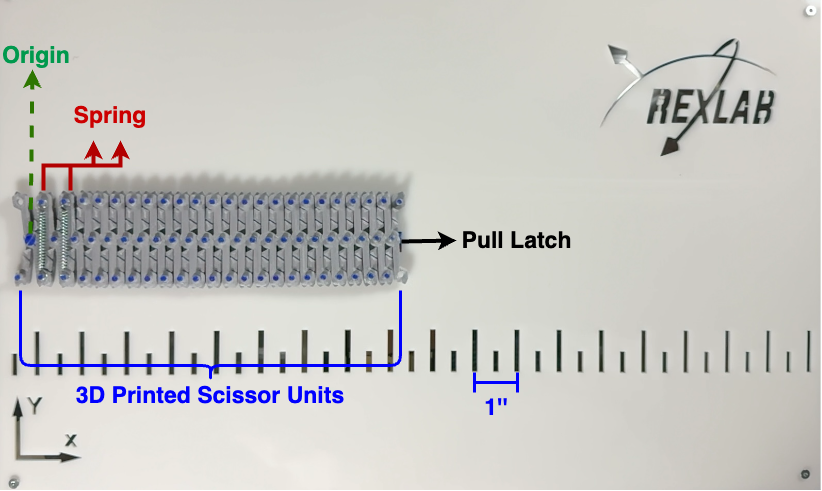
\includegraphics[width=\linewidth]{DOJO-CCK/Figures/scissor_hardware_setup.drawio.png}
    \caption{Hardware experimental setup with a 23-link scissor mechanism with joint clearance and friction. The mechanism has $n$ hook-law extension springs placed at the first $n$ cells of the scissor mechanism. A pull latch sets the mechanism under repeatable conditions, and an overhead high-speed camera captures the motion at 240 fps. The center and end locations of the scissor units are colored in blue to be detected using offline vision segmentation.}
    \label{fig:enter-label}
\end{figure}

\subsection{Simulation-to-Simulation Evaluation}

The digital twin framework was first evaluated using synthetic data in a simulation-to-simulation validation. The experiment comprised a 10-unit scissor mechanism with 0.001m joint tolerance and 0.01 N/m joint friction. This synthetic data served as ground truth for evaluating our estimation methods from visual data error estimation and system parameter identification. This experiment aimed to validate the accuracy of our estimation techniques in a controlled, noise-free environment before applying them to real hardware.

\subsubsection{Hardware Experiment}

A 3D-printed 23-unit scissor mechanism was analyzed to evaluate the efficacy on hardware data. The mechanical system was manufactured using PLA material on a Bambu FDM 3D printer. Springs were added at predefined locations to apply a known opening force, simulating real-world loading conditions. A laser-cut bed with measurement markers created a repeatable experiment environment. The motion of the scissor mechanism was captured using a slow-motion camera at 240 fps. The test bed was equipped with visual markings to convert pixel measurements into meters, facilitating data transfer from the hardware experiment to the simulation. 

% \subsection{Manufacturing and Physical Properties}

% The mechanical system was manufactured using PLA material on a Bambu FDM 3D printer. While the CAD model accurately captures geometrical and inertial properties, it fails to account for joint clearance and joint friction—parameters that can vary during manufacturing. These physical properties were measured and estimated after manufacturing to improve simulation accuracy.
% \subsection{Hardware Experiments with 3D Printed Mechanisms}

% Next, we conducted hardware experiments using 3D-printed versions of the scissor mechanism and the Bennett linkage. Each mechanism was evaluated using distinct experimental setups tailored to capture relevant kinematic and dynamic data.

% \subsubsection{Bennett Linkage Experiment}

% We also printed a 3D Bennett linkage fitted with motion capture markers placed on the coupler bar to track its motion. The linkage was actuated using a stepper motor controlled by an Arduino, operating at a fixed rotational speed of 5 revolutions per minute (RPM). The linkage movement was tracked using an Opti-Track motion capture system, providing high-fidelity position and orientation data for each moving part of the mechanism. This setup enabled the analysis of both kinematic parameters, such as joint clearance, and dynamic parameters, such as joint friction, based on the mechanism's real-world behavior.

% \subsubsection{Digital Twin Identification and Validation}

% The data was integrated into our digital twin framework after estimating the joint clearance and friction from the hardware experiments. The digital twins were validated by comparing the simulation outputs with the hardware measurements under known loading conditions. This comparison allowed us to assess how accurately the digital twin could replicate the physical system's performance.

\subsubsection{Jamming Experiments and Joint Reaction Force Analysis}
Finally, the observed jamming behavior on the hardware was analyzed using the digital twin. The analysis explores the system conditioning over time to the point of jamming and the joint reaction forces. The following section provides a discussion about the results. 

% were analyzed using the digital twins from the prior experiments. These conditions involved applying various forces and torques to simulate real-world scenarios where jamming might occur. We used the slow-motion camera and motion capture system to monitor and record any occurrences of jamming. In the digital twin, we tracked the appearance of additional singular values in the SVD-based model reduction, signaling a loss of degrees of freedom and the onset of jamming. By comparing the digital twin's predictions with real-world outcomes, we validated its ability to detect and analyze jamming behavior under different circumstances.

%%%%%%%%%%%%%%%%%%%%%%%%%%%%%%%%%%%%%%
\section{Results} \label{results}
%%%%%%%%%%%%%%%%%%%%%%%%%%%%%%%%%%%%%%
% \begin{figure}
%     \centering
%     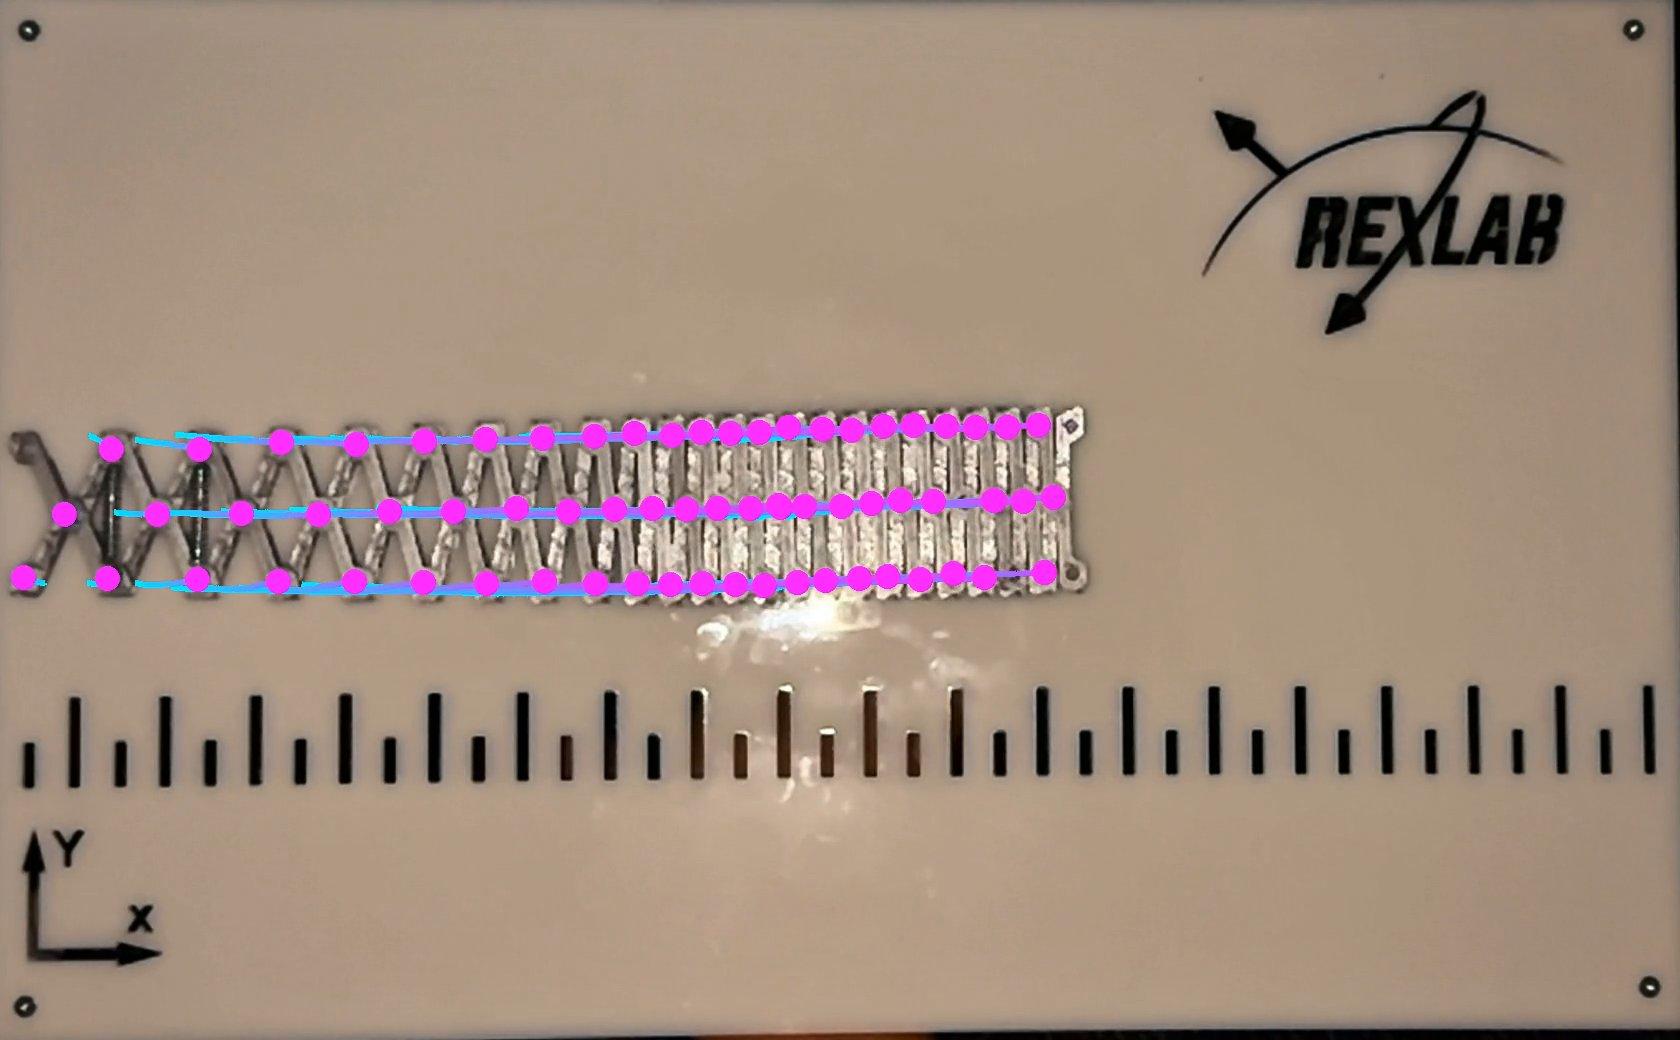
\includegraphics[width=\linewidth]{DOJO-CCK/Figures/Image_scissor_tracking.png}
%     \caption{Caption}
%     \label{fig:enter-label}
% \end{figure}
\begin{figure}
    \centering
    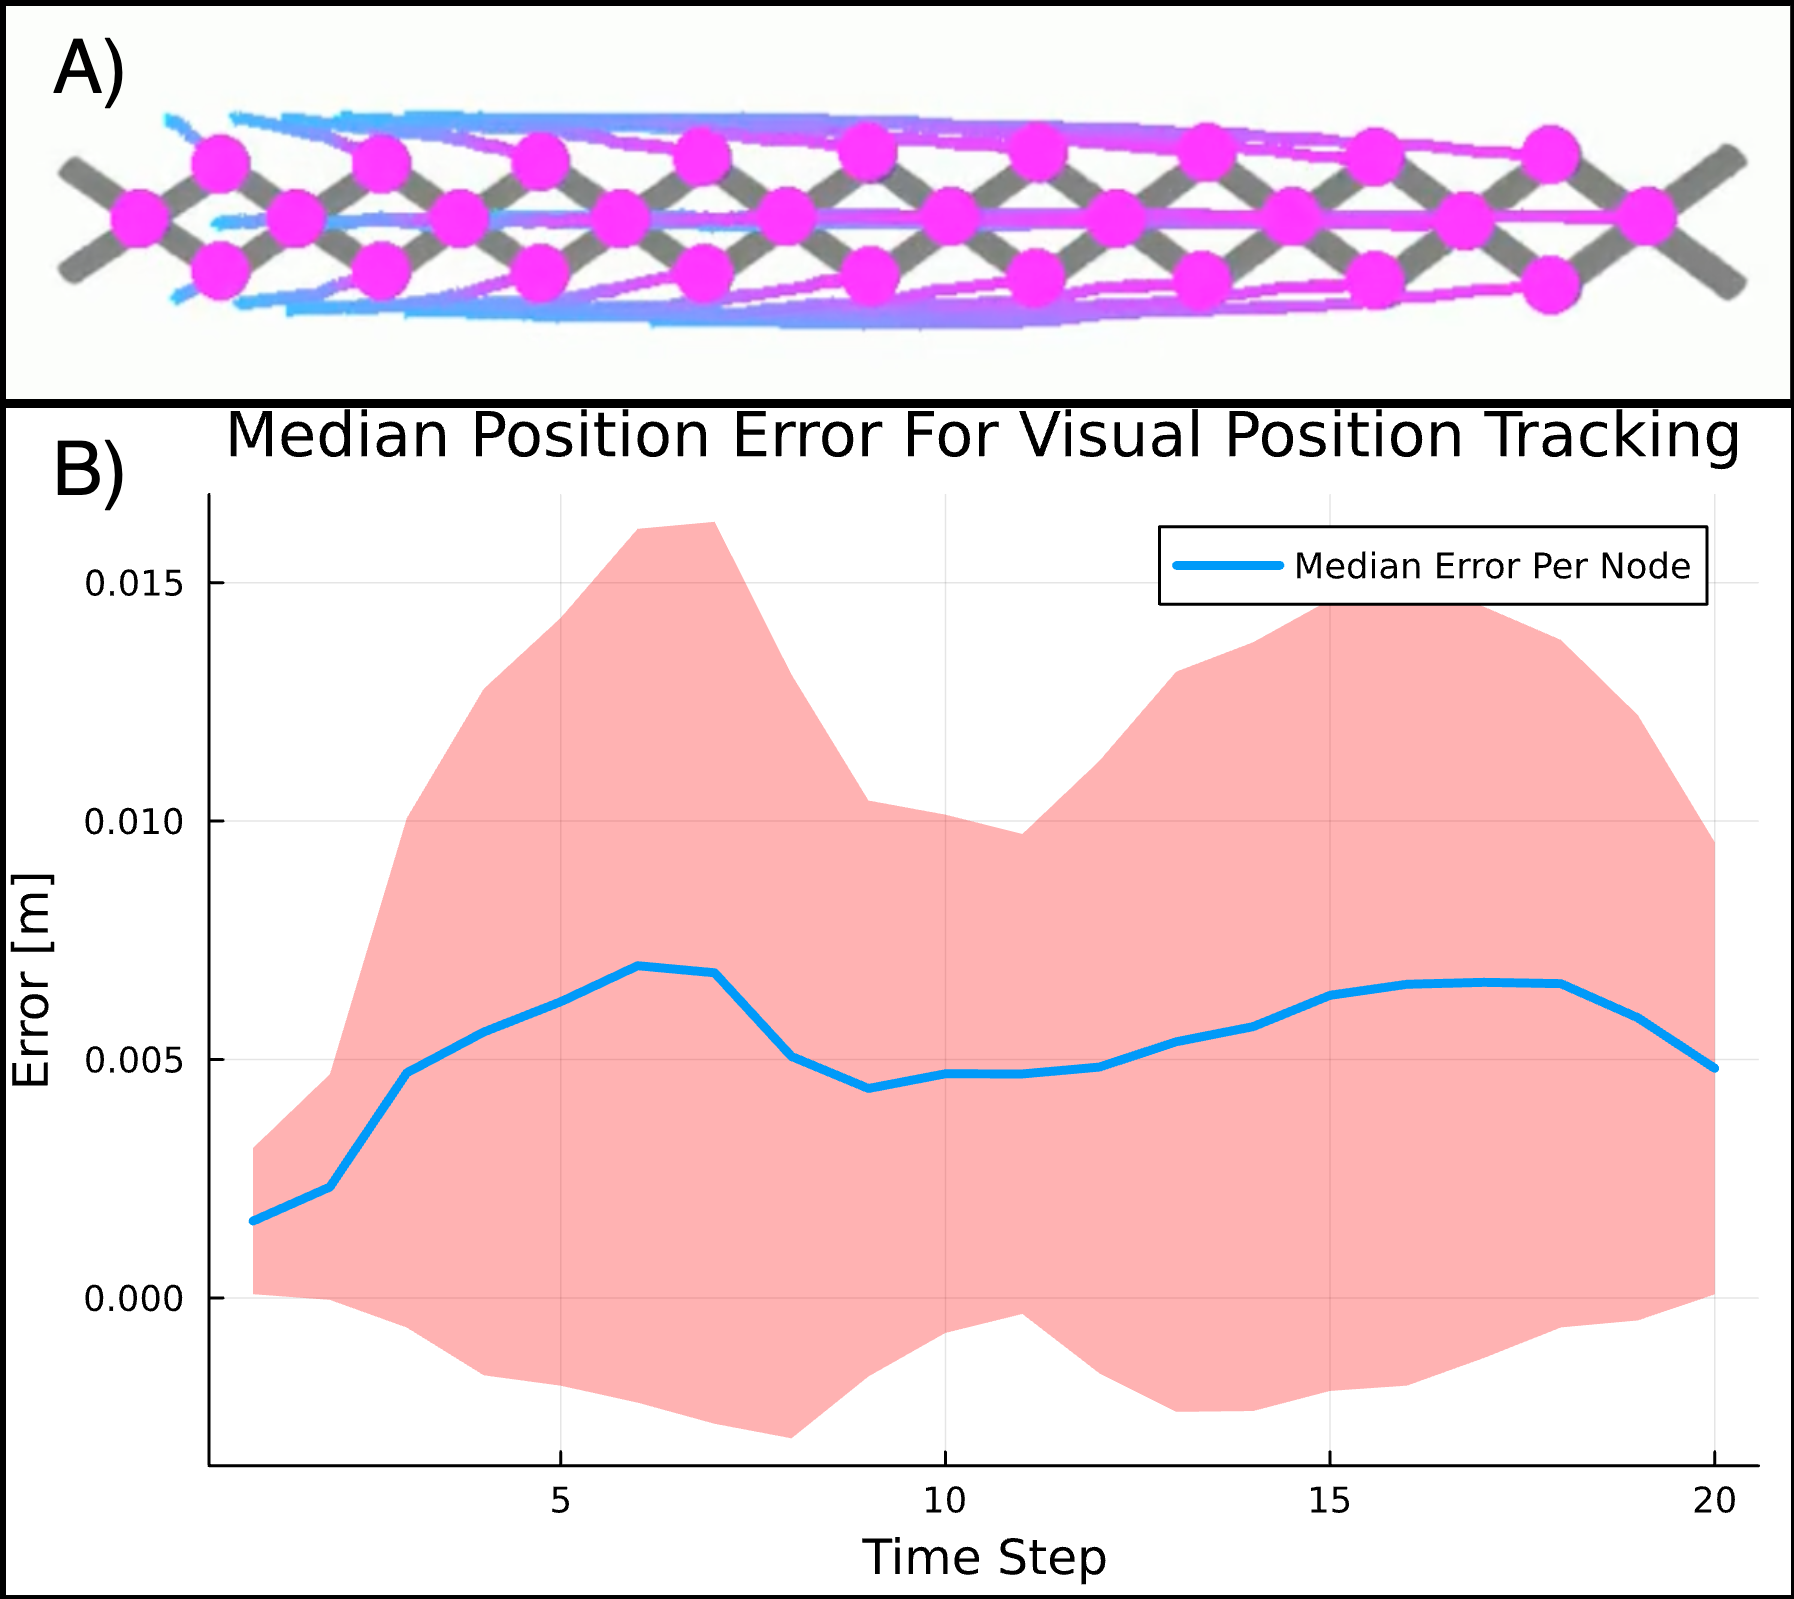
\includegraphics[width=\linewidth]{DOJO-CCK/Figures/tracking_error.drawio.png}
    \caption{ (A) Visual tracking result of the co-tracker on the synthetic scissor mechanism, with tracked points indicated in pink and position history tails. (B) Median position error for visual tracking from ground truth synthetic data per node per time step. The blue line represents the median error per node across each time step, and the shaded red region indicates the range of error variation using median absolute error.}
    \label{fig:sim_to_sim-tracking}
    
\end{figure}
\begin{figure}
    \centering
    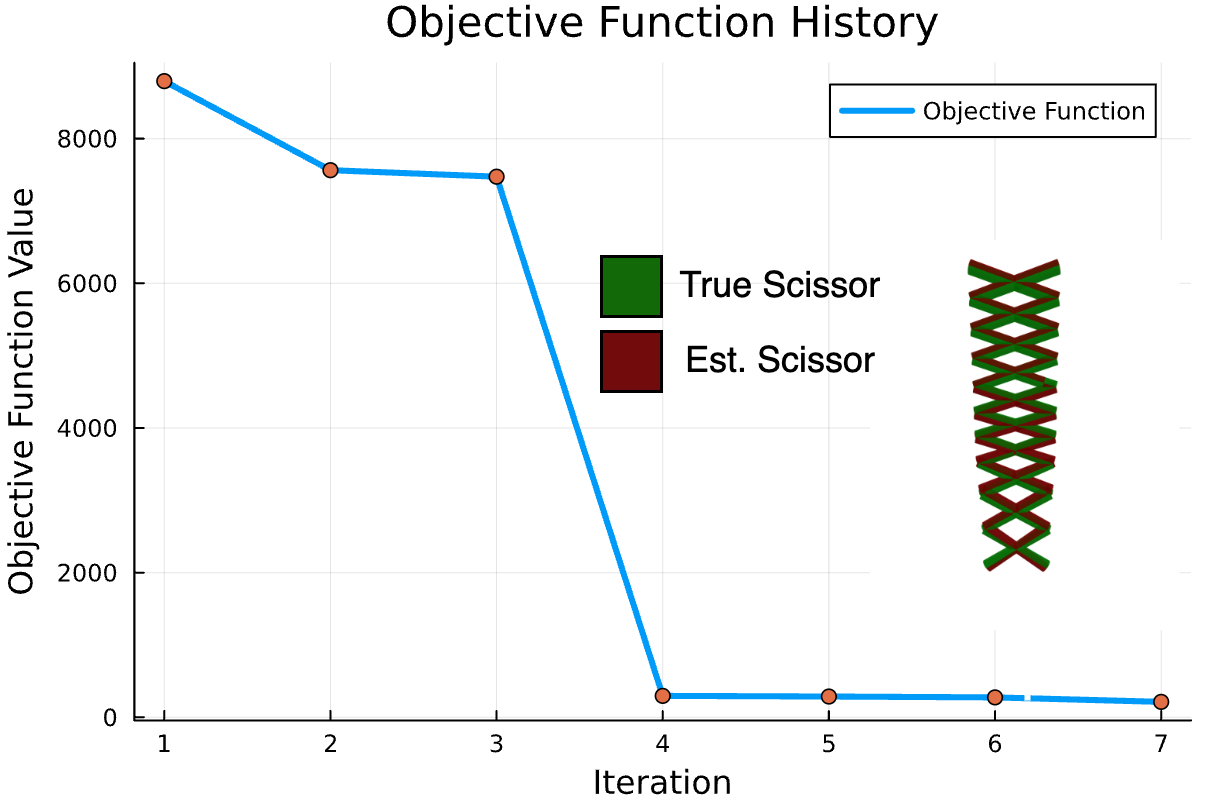
\includegraphics[width=\linewidth]{DOJO-CCK/Figures/simulation_to_simulation_sys_id.drawio.png}
    \caption{Objective function history from LBFGS algorithm for joint clearance and friction estimation, comparing synthetic data with estimated data. The plot shows the objective function value decreasing over iterations as the estimated scissor mechanism (in red) converges to match the true scissor mechanism (in green).}
    \label{fig:sim_to_sim-LBFGS}
\end{figure}
\begin{figure}
    \centering
    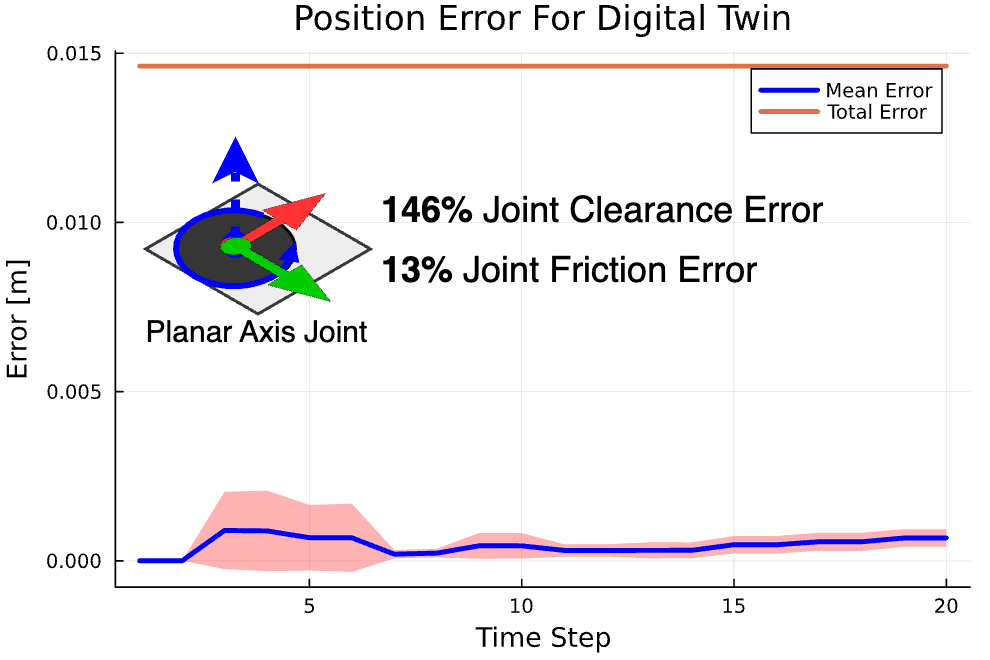
\includegraphics[width=\linewidth]{DOJO-CCK/Figures/simulation_to_simulation_error.drawio.png}
    \caption{Position error for the digital twin, showing the mean error (blue line) and total error (red line) over all time steps. The solution had a 146\% joint clearance error and a 13\% joint friction error. The shaded region represents the variability in position error across time.}
    \label{fig:sim_to_sim-Error}
\end{figure}
\subsection{Synthetic Data results results}
\subsubsection{Visual Analysis}
We evaluate the co-motion optical tracking program using synthetic data generated by our physics engine. The co-motion model was given a pixel mask where joint locations were in the last frame, and the system returned the positions for all video frames. The result of the synthetic data tracking can be seen in Figure \ref{fig:sim_to_sim-tracking} A. These results were then compared with the true joint locations, and the median position error over 20 timesteps is shown in Figure \ref{fig:sim_to_sim-tracking} B. The per-node frame error had a median value of around 5 millimeters. Given that the joint slop to generate the synthetic data was around 1 millimeter, this visual tracking does not provide an ideal resolution for this particular application. Higher-resolution state estimation methods like fiducial markers will be explored in future work. 

\subsubsection{System Identification}
Next, we evaluated the joint optimization from \eqref{eq:optim} using idealized data generated from the physics engine. Equation \eqref{eq:optim} is solved using the LBFGS algorithm. The convergence of the parameters is shown in Figure \ref{fig:sim_to_sim-LBFGS}, and the final parameter error is seen in Figure \ref{fig:sim_to_sim-Error}. While the solution converges to a sub-optimal state with 146\% error in the joint clearance estimate and 13\% error in the joint friction, the overall error over the trajectory is quite low. The joint optimization of these coupled parameters makes the optimization problem challenging, as combinations of joint clearance and friction can provide similar behaviors across the trajectory. Some future directions are to find ways to decouple the optimization or include more data in various loading conditions to better solve for these parameters. 

\begin{figure*}
    \centering
    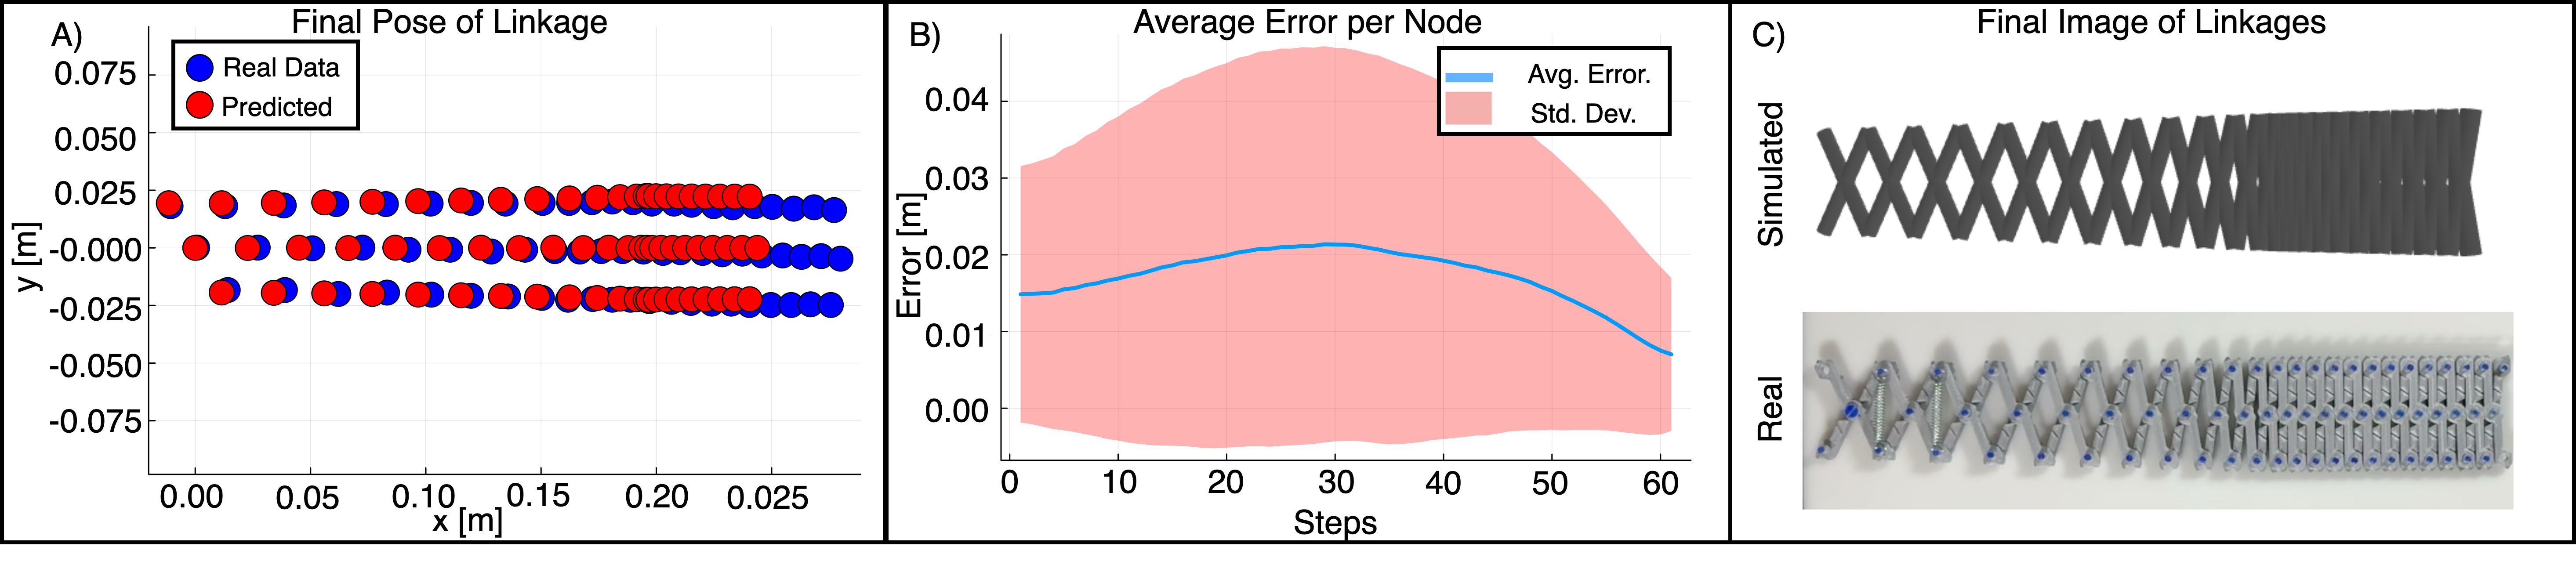
\includegraphics[width=\linewidth]{DOJO-CCK/Figures/hardware_to_simulation_results.drawio.png}
    \caption{Comparison of real vs. simulated positions for the scissor mechanism. (A) The final pose of the linkage, showing real (red) and simulated (blue) positions of the scissor mechanism nodes. (B) Average error per node over time steps, with the blue line representing the mean error and the shaded red area indicating error variation. (C) Final images of the linkage: the top shows the simulated model, while the bottom displays the real-world scissor mechanism. This comparison qualitatively highlights the system’s ability to replicate real-world motion in simulation.}
    \label{fig:real_results}
\end{figure*}
\begin{figure}
    \centering
    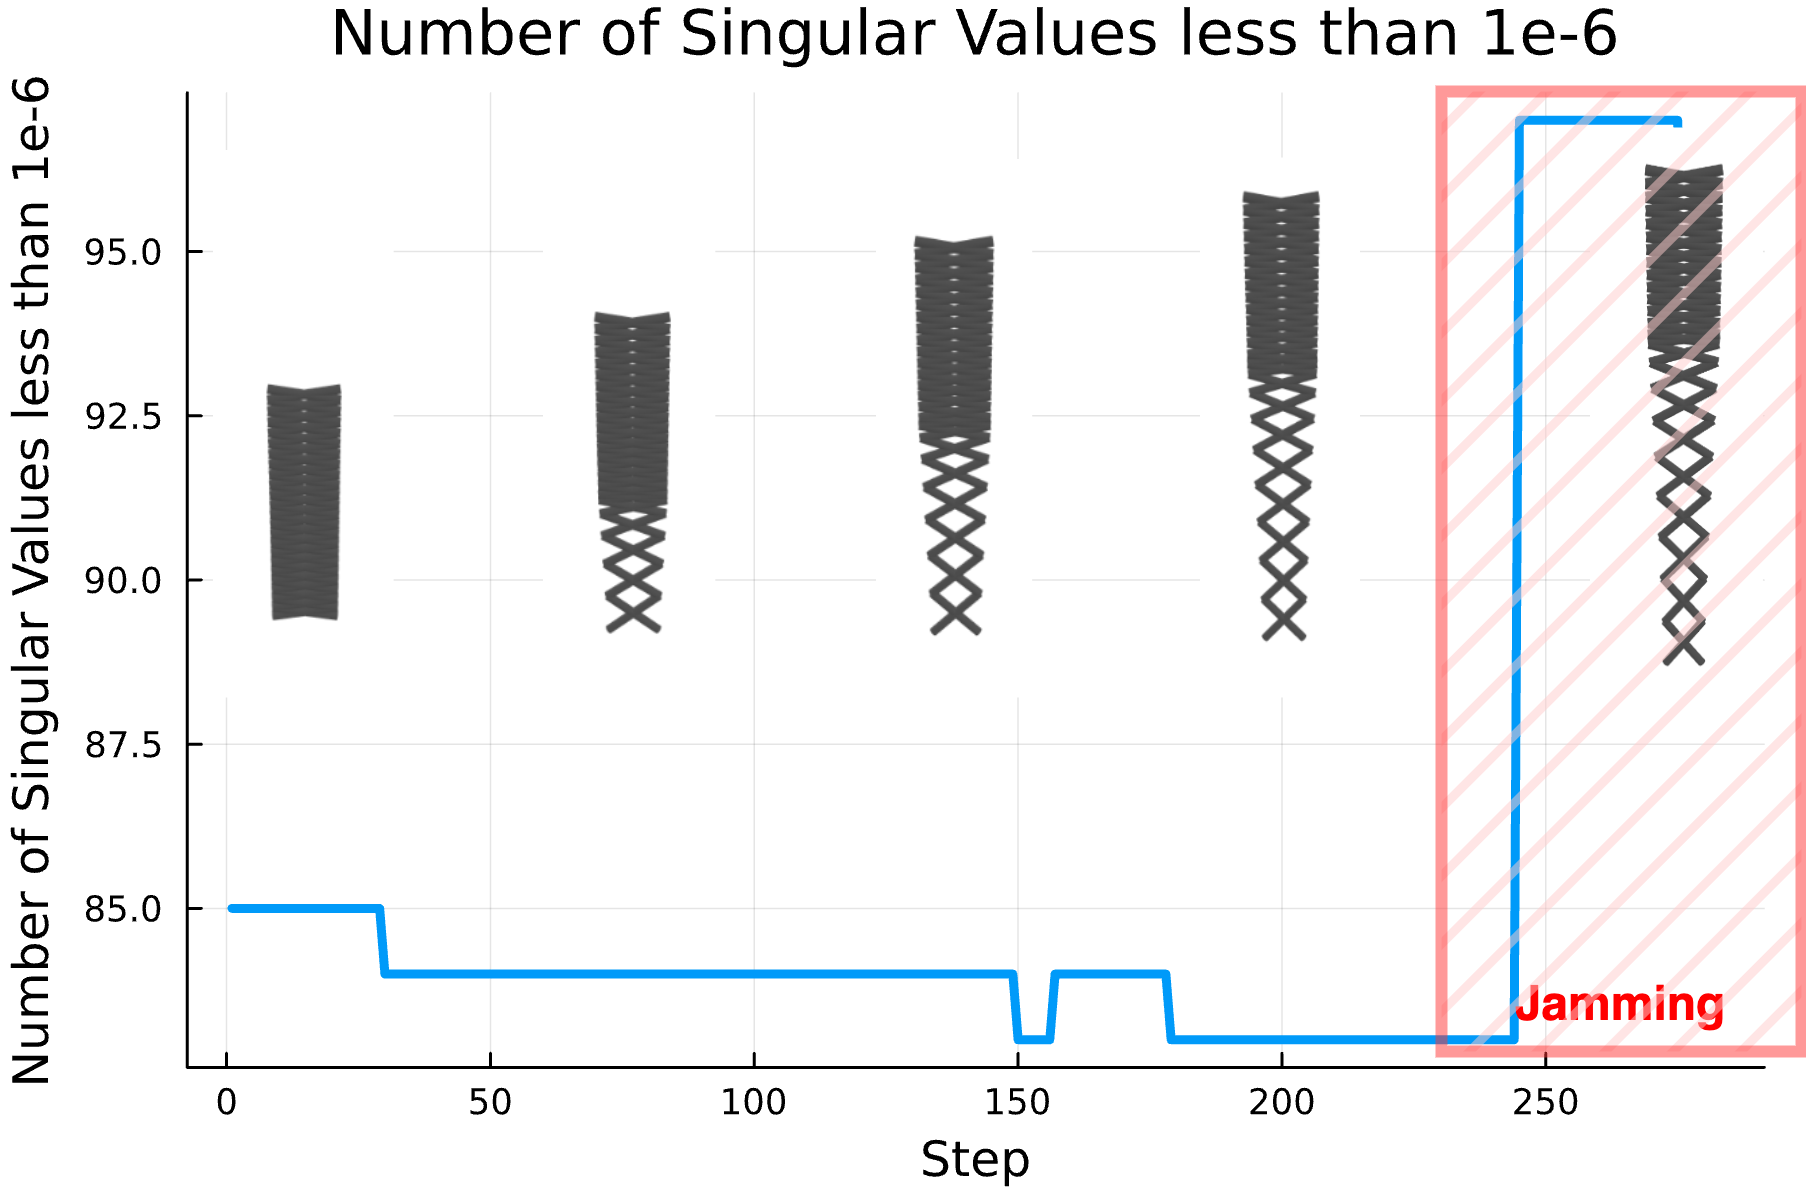
\includegraphics[width=\linewidth]{DOJO-CCK/Figures/Jamming_svds.drawio.png}
    \caption{Singular Value Decomposition (SVD) of the mechanism under loading conditions, showing the number of singular values less than 1e-6 over time steps. The increase in the number of small singular values indicates the onset of jamming (highlighted in the red-shaded region).}
    \label{fig:jamming-detection}
      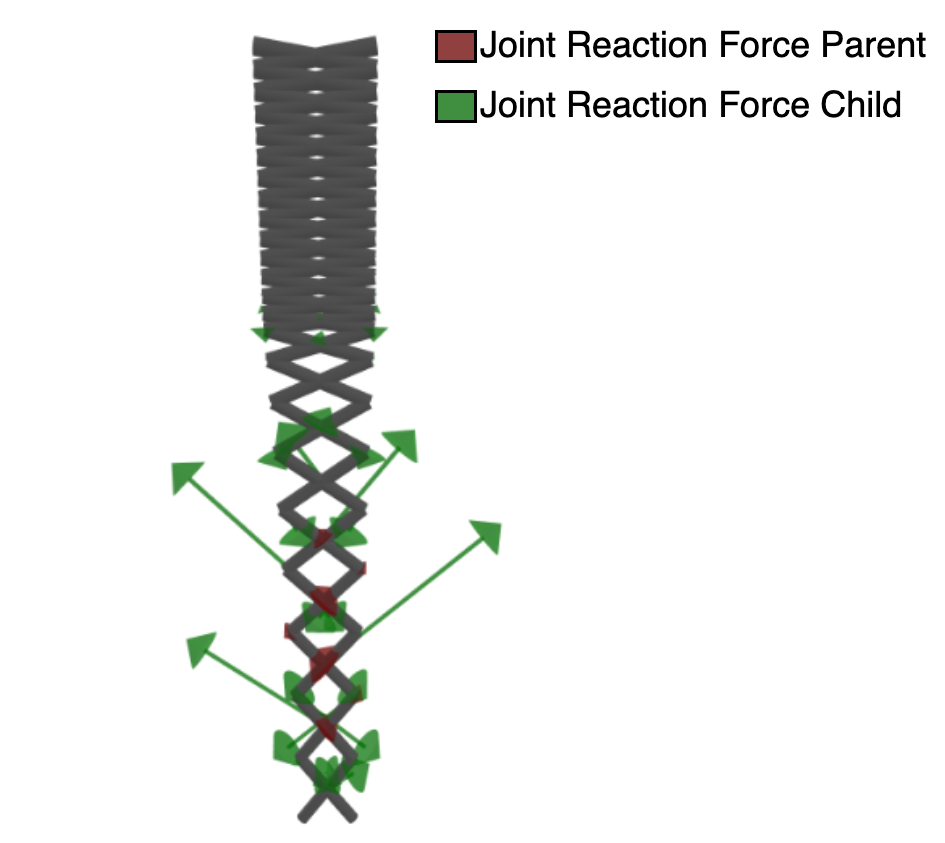
\includegraphics[width=\linewidth]{DOJO-CCK/Figures/joint_reaction_forces.drawio.png}
    \caption{Visualization of joint constraint forces during jamming. The arrows represent joint reaction forces, with red indicating forces on the parent link and green showing forces on the child link. }
    \label{fig:constraint-force}
\end{figure}
% \begin{figure}
%     \centering
%     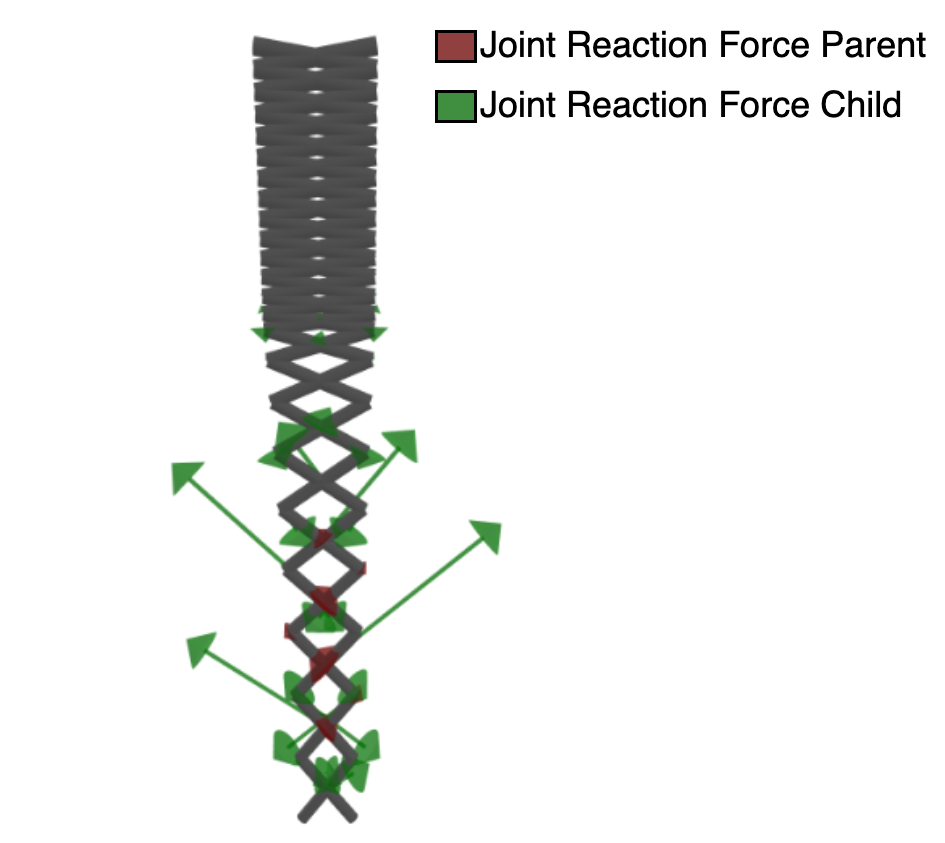
\includegraphics[width=\linewidth]{DOJO-CCK/Figures/joint_reaction_forces.drawio.png}
%     \caption{Visualization of joint constraint forces during jamming. The arrows represent joint reaction forces, with red indicating forces on the parent link and green showing forces on the child link. }
%     \label{fig:constraint-force}
% \end{figure}
\subsection{Hardware experiment results}
Initial experimentation was also performed on a 23-unit scissor mechanism. The mechanism is driven using two extension springs with a Spring force of 2870 N/m. The springs fail to deploy this linkage completely due to the joint clearance and friction. The positions of the joint locations are extracted using the OpenCV and co-tracker packages. We can assume a median error per node around 5 mm from the synthetic data experiment. The true values for the joint clearance are estimated by measuring using calipers to be around 0.4 mm. The true joint friction cannot be directly measured to provide a ground truth. The results for the hardware experiment can be seen in Figure \ref{fig:real_results}. We found that the best joint friction was around 0.003 Ns/m, and we fixed the joint clearance to a value of 0.4mm based on the true measurement. Figure \ref{fig:real_results}A shows the tracked locations from the real and simulated results. Figure \ref{fig:real_results}B shows the average error per node per time step, which is between 1-2 cm. This value is quite reasonable given that the resolution of the visual measurement is $\pm$5mm. Finally, Figure \ref{fig:real_results}C compares the simulated and real hardware qualitatively. This image shows that the joint limits on this simulated version do not match that of the real hardware, as the scissors are packing much tighter in the non-extended region. This could account for the position error between the simulated and real systems. These initial results are promising for future digital twin generation of linkage mechanisms and provide an interesting challenge for measurement resolution to capture joint tolerances. 
% TODO: Scissor Mechanism Position Tracking:
% % Present the real-world position tracking data from the slow-motion camera compared to the simulated positions from the digital twin.
% % Discuss any discrepancies between the simulated and real-world data, particularly in the context of joint clearance and friction.
% % Plot/Table: Real vs. simulated positions for the scissor mechanism.
% TODO: Bennett Linkage Position Tracking:
% % Show the real-world tracking data for the Bennett linkage using the motion capture system, compared to the simulation results.
% % Highlight how the digital twin captures the dynamics of the linkage and compare the joint clearance and friction estimations.
% % Plot/Table: Real vs. simulated positions for the Bennett linkage.

\subsection{Jamming Detection}
Finally, jamming and joint force analysis were explored using the above model. Jamming is a phenomenon in linkages that are frequently seen in hardware but under-explored in simulation modeling. This is likely due to the ill-conditioning that occurs when jamming takes place. Figure \ref{fig:jamming-detection} shows the number of singular values lower than 1e-6 over a 275-step deployment of the linkage. For most of the linkage deployment, the number of singular values stays around constant or decreases, likely due to numerical limitations. At step 250, the number of singular values sharply increases for several steps until the end of the simulation. This sharp increase in singular values means fewer degrees of freedom for the system to move in. The joint constraint forces are shown in Figure \ref{fig:constraint-force} with the forces acting on the child nodes of the constraint shown in green and the parent nodes in red. Further investigation on the significance of the magnitude and direction of the constraint forces is needed to better characterize why jamming occurs at this point in the deployment. 
% TODO: Jamming Detection Results
% Simulation Behavior Under Different Loading Conditions:
% Present the results from simulations with various loading conditions designed to induce jamming in both the scissor mechanism and Bennett linkage.
% Discuss the appearance of additional singular values in the SVD-based model reduction during jamming events.
% Show how the increase in thresholded singular values indicates a reduction in the degrees of freedom, correlating with the onset of jamming.
% Plot: Singular values under normal and jamming conditions
% Joint Constraint Forces During Jamming:
% Present the results of the simulation forces experienced by the joints during jamming events.
% Discuss how the digital twin captures the increase in constraint forces as the system jams, providing insights into mechanical limits.
% Figure: Visualization of joint constraint forces during jamming.





% TODO: TABLE Estimated Joint Clearance and Friction (Scissor Mechanism and Bennett Linkage)



%%%%%%%%%%%%%%%%%%%%%%%%%%%%%%%%%%%%%%
\section{Conclusions} \label{conclusion}
%%%%%%%%%%%%%%%%%%%%%%%%%%%%%%%%%%%%%%
In this paper, we developed a new framework for a data-driven, physics-based digital twin for linkage analysis, incorporating joint clearance and joint friction estimation. We demonstrated the digital twin's current capabilities and limitations in replicating real-world mechanisms through simulation-to-simulation and hardware experiments. The ability to identify jamming and capture joint constraint forces through the physics engine with SVD factorization is of particular interest. Future work will investigate the jamming behavior and design features that can help mitigate this problem. While the current study assumes uniform joint clearance and focuses on revolute and fixed joints, future work will expand the model to support additional joint types and improve the automatic threshold selection for SVD truncation. Future research will also involve testing the digital twin framework in more complex and real-world scenarios to enhance its capabilities. Overall, this work is the first step in next-generation tools for space-based deployable structure design to be more effective and efficient with a higher chance of mission success.
%%%%%%%%%%%%%%%%%%%%%%%%%%%%%%%%%%%%%%%%%%%%%%%%%%%%%%%%%%%%%%%%%%%%%%%%%%%%%%%%%%%%%%%%%%%%%%%%%
% \appendices{}              % note there is no {} to put a title. Each appendix has its own title
%%%%%%%%%%%%%%%%%%%%%%%%%%%%%%%%%%%%%%%%%%%%%%%%%%%%%%%%%%%%%%%%%%%%%%%%%%%%%%%%%%%%%%%%%%%%%%%%%
% For a single appendix, use the \appendix{} keyword and do not use the \section command.

% \input{DOJO-CCK/Sections/Appendix}
%%%%%%%%%%%%%%%%%%%%%%%%%%%%%%%%%%%%%%%%%%%%%%%%%%%%%%%%%%%%%%%%%%%%%%%%%%%%%%%%%%%%%%%%%%%%%%%%%%%%%%
\acknowledgments{This work was supported by a NIAC award from NASA’s Space Technology Mission Directorate (Grant Number 80NSSC22K0767). The authors would like to acknowledge Jan Bruedigam for helping with Dojo simulation debugging, Arun Bishop and John Zhang for useful discussions, Sawyer Thomas who designed the scissor mechanism used in this work, and Walter Holzwarth, whose CAD of the Bennett linkage we modified for the paper.}
%%%%%%%%%%%%%%%%%%%%%%%%%%%%%%%%%%%%%%%%%%%%%%%%%%%%%%%%%%%%%%%%%%%%%%%%%%%%%%%%%%%%%%%%%%%%%%%%%%%%%%
% \bibliographystyle{IEEEtran}
\printbibliography %Prints bibliography

% \begin{thebibliography}{1}
% \bibliography{DOJO-CCK/DOJO_CKC_IEEE_AERO}
% \thebiography

% \bibitem{ITAR}
% U.S. Munitions List, Sections 38 and 47(7) of the Arms Export Control Act (22 U.S.C 2778 and 2794(7).

% \bibitem{AeroConf}
% Aerospace Conference Web site: \underline{www.aeroconf.org}.

% \end{thebibliography}


%%%%%%%%%%%%%%%%%%%%%%%%%%%%%%%%%%%%%%%%%%%%%%%%%%%%%%%%%%%%%%%%%%%%%%%%%%%%%%%%%%%%%%%%%%%%%%%%%%%%%%
% \thebiography
% \bibliographystyle{splncs04}
% \bibliography{}
%% This biostyle allows you to insert your photo size 1in X 1.25in
\begin{biographywithpic}
    {Mitchell Bennett Fogelson}{DOJO-CCK/Figures/headshot_skinny.jpg} received his B.S.E and M.S.E from the University of Pennsylvania in Mechanical Engineering in 2017 and Robotics in 2018 respectively. He is currently a Ph.D. candidate in Mechanical Engineering from Carnegie Mellon University. His research includes advanced simulation and optimization methods for mechanical metamaterials and robotic systems.
\end{biographywithpic} 


\begin{biographywithpic}
    {Zachary Manchester}{DOJO-CCK/Figures/Zac-Headshot-IEEE.png} %pic
    is an assistant professor in the Robotics Institute at Carnegie Mellon University and founder of the Robotic Exploration Lab. He received a PhD in aerospace engineering in 2015 and a BS in applied physics in 2009, both from Cornell University. His research interests include control and optimization with applications to aerospace and robotic systems. 
\end{biographywithpic}




\end{document}
